\documentclass[10pt,showpacs,preprintnumbers,footinbib,amsmath,amssymb,aps,prl,twocolumn,groupedaddress,superscriptaddress,showkeys]{revtex4-1}
\usepackage{graphicx}
\usepackage{dcolumn}
\usepackage{bm}
\usepackage[colorlinks=true,urlcolor=blue,citecolor=blue]{hyperref}
\usepackage{color}
\usepackage{listings}
\usepackage{subfig}

\lstset{ %
  basicstyle=\footnotesize,        % the size of the fonts that are used for the code
  breakatwhitespace=false,         % sets if automatic breaks should only happen at whitespace
  breaklines=true,                 % sets automatic line breaking
  captionpos=t,                    % sets the caption-position to bottom
  deletekeywords={...},            % if you want to delete keywords from the given language
  escapeinside={\%*}{*)},          % if you want to add LaTeX within your code
  extendedchars=true,              % lets you use non-ASCII characters; for 8-bits encodings only, does not work with UTF-8
  frame=single,                    % adds a frame around the code
  keepspaces=true,                 % keeps spaces in text, useful for keeping indentation of code (possibly needs columns=flexible)
 % language=Python,                 % the language of the code
  morekeywords={*,...},           % if you want to add more keywords to the set
  numbers=left,                    % where to put the line-numbers; possible values are (none, left, right)
  numbersep=5pt,                   % how far the line-numbers are from the code
  showspaces=false,                % show spaces everywhere adding particular underscores; it overrides 'showstringspaces'
  showstringspaces=false,          % underline spaces within strings only
  showtabs=false,                  % show tabs within strings adding particular underscores
  stepnumber=1,                    % the step between two line-numbers. If it's 1, each line will be numbered
  tabsize=2,                       % sets default tabsize to 2 spaces
}


\begin{document}
\title{FYS3150 Computational Physics - Project 3}
\author{Nicholas Karlsen}

\begin{abstract}
This is an abstract
\end{abstract}

\maketitle

\section{Introduction}
  
  Lastly, the source code for any code discussed in this report can be found on my
  Github at: \url{https://github.com/nicholaskarlsen/FYS3150}

\section{Theory, Algorithms and Methods}
  
  \subsection{Discretizing Newton's law of universal gravitation}
    Between every body, there is a force of attraction inversly proportional to the square of the separation, or more precisely, the force acting on some body with mass $m$ due to a mass $m'$ is
    \begin{equation}
      \mathbf F = G\frac{m m'}{|\mathbf r - \mathbf r'|^2}\mathbf{\hat{u}_{r-r'}}, \quad \mathbf{\hat{u}_{r-r'}} = \frac{\mathbf r - \mathbf r'}{\mathbf |\mathbf r - \mathbf r'|}
    \end{equation}
    Where $G$ is the gravitational constant and $\mathbf r$ denotes the vector from the body of mass $m$ to mass $m'$

    If we choose to work in the cartesian coordinate system centered on the body with mass $m'$, then $\mathbf r = -(x, y, z)$ and $|\mathbf r| = \sqrt{x^2 + y^2 + z^2} = r$.

    By Newtons second law, the acceleration on body 1 due to the gravitational pull of body 2 can then be written as
    \begin{equation}
      \mathbf a = \frac{1}{m}\mathbf F = G \frac{m'}{r^2}\frac{\mathbf r}{r} = -G\frac{m'}{r^2}\frac{\left(x, y, z\right)}{r}
    \end{equation}
    Written out component-wise in terms of the positions, we get the set of coupled differential equations

    \begin{equation}
      \frac{\partial x^2}{\partial t^2} = -G\frac{m'}{r^2}\frac{x}{r}, \quad
      \frac{\partial y^2}{\partial t^2} = -G\frac{m'}{r^2}\frac{y}{r}, \quad
      \frac{\partial z^2}{\partial t^2} = -G\frac{m'}{r^2}\frac{z}{r}
    \end{equation}


\begin{lstlisting}[mathescape=true, language=python, title=Euler-Cromer Algorithm]
for $i = 0, \dots, N-1$
    $\mathbf v_{i + 1} = \mathbf v_{i} + \mathbf a_{i}\Delta t$
    $\mathbf r_{i + 1} = \mathbf r_{i} + \mathbf v_{i + 1}$
\end{lstlisting}

\begin{lstlisting}[mathescape=true, language=python, title=Velocity-Verlet Algorithm]
for $i = 0, \dots, N-1$
  $\mathbf r_{i+1} = \mathbf r_i + \mathbf v_i \Delta t + \frac{1}{2}\mathbf a_i(\Delta t)^2$
  $\mathbf v_{i+1} = \mathbf v_i + \frac{1}{2}(\mathbf a_{i+1} + \mathbf a_i)\Delta t  $
\end{lstlisting}

\section{Results and Discussions}

\begin{figure}[h!tb]
  \center
  \subfloat[][Velocity-Verlet]{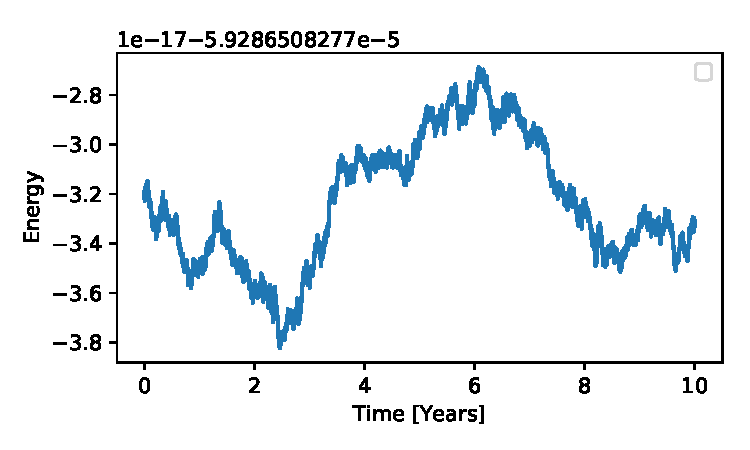
\includegraphics[width=8cm]{figs/exb_energy_verlet.pdf}\label{fig:earthsun energy verlet}}\\
   \subfloat[][Euler-Cromer]{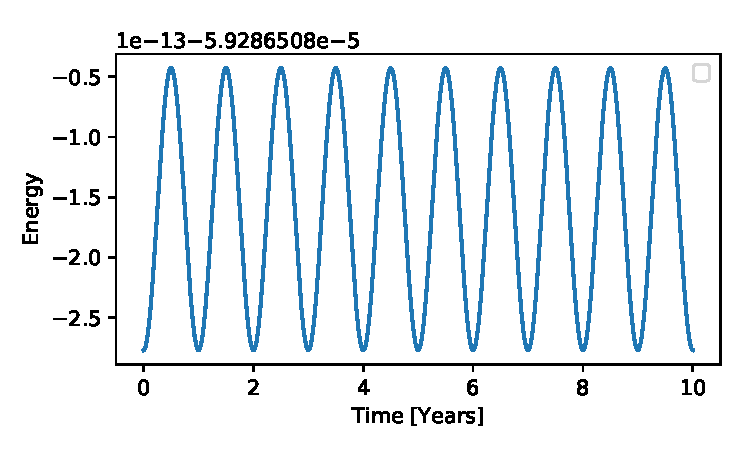
\includegraphics[width=8cm]{figs/exb_energy_euler.pdf}\label{fig:earthsun energy cromer}}
   \caption{The fluctuation of the total energy of the Earth in the Earth-Sun system for solutions using the Velocity-Verlet algorithm (a) and the Euler-Cromer algorithm (b)}
   \label{steady_state}
\end{figure}

\begin{figure}[h!tb]
  \center
  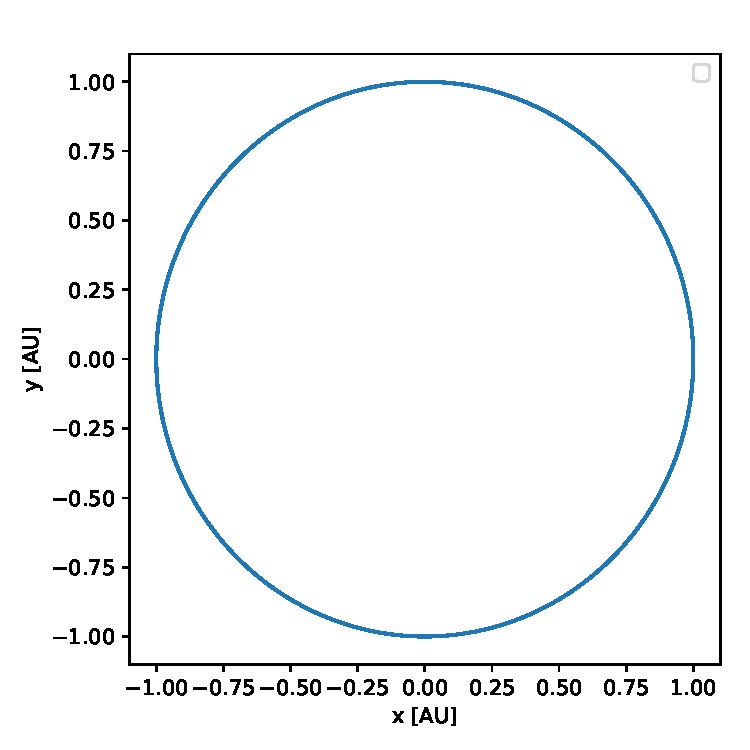
\includegraphics[width=8cm]{figs/exb_orbit_verlet.pdf}
\end{figure}



\section{Conclusions}
  In trying to generalize my code through the use of object orientation, i had to strike a balance between generality and complexity

\begin{thebibliography}{99}
\bibitem{lecture_notes} M.~Hjorth-Jensen, Computational Physics - Lecture Notes 2015, (2015).
\end{thebibliography}

\appendix
\section{Fetching data from Horizons using horizons.py}
  In order to streamline the process of fetching data from the Horizons system i created a small script, \lstinline{horizons.py} that utilizes the Astroquery python package and returns only the select data that i am interested in. The function, \lstinline{fetch_data} takes input as a dictionary, rather than a list of id numbers. Whilst this may not be as extensible or practical, it makes the code easier to read and understand, by making the instant connection between the planet name and id. For the purposes of this project, i find that much more valuable since i am only dealing with a limited amount of planets anyway.
\end{document}  